\documentclass[12pt]{iopart}
%\documentclass[12pt]{article}

\usepackage{amstext}
\usepackage{amssymb}
\usepackage{graphicx}
\usepackage{color}
\usepackage{subfigure}
\usepackage[colorlinks=true]{hyperref}
\usepackage{../../../bibtex/aas_macros}

\begin{document}

\title[] {Optimizing Deep Searches for Gravitional waves from Binary Coalescance} 
\author{Alexander H. Nitz$^1$, Joshua L. Willis$^2$, Ian W. Harry$^4$, Andrew Lundren$^3$, Tito Dal Canton$^3$, Larne Pekowsky$^1$, Duncan A. Brown$^1$}
\address{$^1$ Syracuse University, Syracuse, NY 13244, USA}
\address{$^2$ Abilene Christian University, Box 27963, Abilene, TX 79699, USA}
\address{$^3$ Max Planck Institut f\"ur Gravitationsphysik, Callinstrasse 38,  D-30167 Hannover, Germany}
\address{$^4$ Max Planck Institut f\"ur Gravitationsphysik, Am Muehlenberg 1,  D-14476 Potsdam, Germany}

\begin{abstract}
\end{abstract}

\section{Introduction}
\label{sec:introduction}

\section{Methods of the Inspiral Search}
\label{sec:search_methods}

Stuff.. \cite{Allen:2005fk}

In this section describe the theoretical costs of the algorithm [{\bfseries Alex
  to provide these calculations}].  In particular, we want theoretical costs
for:
\begin{enumerate}
\item Direct matched-filtering using the inverse FFT to calculate the
  convolution as a function of coalescence time (as is done now).
\item Singular value decomposition, in both the time and frequency domains.
\item Basic steps before and after the convolution: correlation of the data and
  template, finding output time series points above the threshold, and
  clustering. The theoretical performance of these steps will presumably be
  bandwidth limited, but we should state (and show) that.
\item The cost of various commonly deployed vetoes, including the ``Bruce'' $
chi^2$, the auto-correlation $\chi^2$, and perhaps the bank $\chi^2$. We may
also here want to discuss the computational cost of alternate algorithmic
implementations of these, to prepare the ground for our later ``future
optimizations.'' (Basically, do we want a detailed theoretical calculation here
of the alternate methods that we are investigating, or does that belong
somehwere else?) 
\end{enumerate}

We should discuss how the original FINDCHIRP algorithm tied together several specific
algorithmic choices, but the current code does (or will) allow separation of
these steps, which will be important both for general optimizations as well as
adapting the optimization to the specific hardware.
\begin{enumerate}
\item Segmenting for PSD estimation.
\item ``Batching'' of the steps of the matched-filter, to allow amortizing of
  latencies between different steps.
\end{enumerate}

\section{Computational Scaling of Inspiral Analysis using Direct FFT matched-filtering}

In this section, we calculate the scaling of floating point operations and memory accesses 
for the direct calculation of the matched-filtering algorithm using an inverse Fourier
transform.


\subsection{Data preconditioning}

The matched-filter operation can be expressed as,

\begin{equation}
\rho(t) = \int  \tilde{h}^{*} (\frac{\tilde{s}}{s_n}) e^{-2\pi if t } df,
\end{equation}

where $\tilde{h}^*$ is the frequency domain complex conjugate template waveform, $\tilde{s}$ is the 
frequency domain strain data, and $s_n$ is the power spectral density. 

At the start of an inspiral program, $T$ seconds of gravitional-wave strain data is read in and 
preconditioned. It broken into $N_s$ analysis segment each of 
length $N$ samples, where $N = l_s / df$. $l_s$ is the number of seconds corresponding 
to each analysis segment and $df$ is the time stepping. These segments are 
are Fourier transformed, divided by the power spectral density $s_n(f)$ to overwhiten them,
and stored in memory for the duration of the program. Each segment is
filtered against $N_t$ template waveforms. The relative cost to generate
each preconditioned analysis segment scales
as $ O(1 / N_t)$. In general, this cost may can be neglected, 
as the typical number of templates is quite large, $N_t0 \approx 10^3 - 10^5$, 
and will grow as Advanced LIGO approaches final design sensitivity. 

\subsection{Template Generation}

Once for every $N_s$ analysis segments, a new template is generated. Where the SPA approximation
applies, the template can be expressed as a polynomial function which can be evaluated directly
in the frequency domain. A template is generated once and filtered against the set of 
precalculated analysis segments. The relative cost scales as the inverse of the 
number of analysis segments, $1 / N_s$. The limiting factor for the number of analysis
segments is the amount of memory required to store them. A typical segment size is 
$2^{23} bytes$. For typical hardware configutations,  storing $O(50)$ segments is possible, 
and so the cost of template generation may be neglected.

\subsection{Segment Tiling}

Filtering in the frequency domain necessarily implies that the correlations are performed
on a circular ring. To remove the corruption caused by wraparound, the leading and tailing
portions of each analysis segment are excised. The segments are then tiled
to ensure full coverage of the gravitational-wave data. The amount of valid analysis
time, $T$, can be expressed n terms of the number of segments, $N_s$, the length
of each segment $l_s$ and the fraction of valid time in each segment $f_v$.

\begin{equation}
 T = N_s * f_v * l_s
\end{equation}

The valid portion of each segment can in turn be epxressed if terms of the length
of the template waveform $l_s$ and the inverse power spectrum $l_{psd}$ in seconds. 

\begin{equation}
 T = N_s * [\frac{l_s-l_{psd}-l_t}{l_s}] *  l_s
\end{equation}

Conversely, the number of segments to tile a given length of time $T$ is expressed as,

\begin{equation}
N_s = \frac{T}{l_s -l_{psd} - l_t}
\end{equation}

Clearly, the number of segments needed to analyze a given time is minimized by increasing 
the length $l_s$ of each analyze segment. However, that this needs to be balanced
agains the performance effects of larger FFT sizes. 

\subsection{Correlation}
The first step in the inner matched filtering loop is to multiply the precalculated
template and overwhitened data segments, expresed as follows. 

\begin{equation}
 \tilde{q} = \tilde{h}^* (\frac{\tilde{s}}{s_n})
\end{equation}

All vectors are length N, single precision, and complex valued. 
Filtering only takes places up to the 
Nyquist frequency at sample $N/2+1$, so it is known that the last half of the output
vector $\tilde{q}$ must be zero. Where the template waveform terminates
below the Nyquist frequency at a value $k_t$, we may take $\tilde{q}$ to be zero beyond
this point. We take $k_{max}$ to be defined as,

\begin{equation}
 k_{kmax} = minimum(N/2, k_t).
\end{equation}

Six floating point operations are required to perform each complex multiplcation and 
conjugation for each of the $k_{max}$ samples per analysis segment. If we take the a 
memory read/write in units of 4 bytes, then the computational requirements of this
step are

\begin{equation}
 FLOP = 6 K_{max}, \\
 READ = 4 K_{max}, \\
 WRITE = 2 K_{max}. 
\end{equation}

It is evident that the ratio of read and write operations is quite high compared the the
floating point operations, indicating that this step is likely memory bandwidth bound.

\subsection{Inverser Fourier Transform}

The vector $\tilde{q}$ is then inverse Fourier transformed to calculate the complex SNR, 
$\rho(t)$, 
We take the conanoncial flaoting point
cost of an FFT to be, 

\begin{equation}
 FLOP = 5 Nlog(N).
\end{equation}

We note that typical FFTs at the size we use are memory-bandwidth bound, but that the 
exact behavior is highly hardware dependent, see section on FFT benchmarking. 

\subsection{Peak Finding}

We locate peaks in our complex signal-to-noise ratio, $\rho(t)$, by taking the 
absolute manitude of each element and thresholding. This requires 3 floating point
operations for taking the magnitude of each element, and 1 for the comparison to 
the threshold, yielding,

\begin{equation}
 FLOP =  4 N, \\
 READ =  2 N, \\
 WRITE = 2 N_p,
\end{equation}

where we define $N_p$ as the number of points above threshold. $N_p$ for a Gaussian
noise source may be modeled as,

\begin{equation}
 N_p \approx e^{-\frac{\rho_t^2}{2}}*N
\end{equation}

where $\rho_t$ is the SNR threshold. Note, that actual LIGO data is not well modeled as 
a coloured Gaussian stream of data. In particular, there are loud glitches, which we
must take care to distinguish from true signals. 

\subsection{Signal-consistency Test}
If points are found above threshold, the a time-frequency signal consistency test is applied.
The test consists of breaking the waveform into $p$ frequency bins of equal power. Each bin is
filtered against the data to obtain the partial SNR contribution $\rho_l$ and then compared to
the expected SNR contribution $\rho \ p$. This is expressed
as

\begin{equation}
 \chi^2 = p \sum_{l=0}^{p} [\rho_l - \rho / p]^2,
\end{equation}

which can be simplified as follows.

\begin{equation}
 \chi^2 = p \sum_{l=0}^{p} \left(\rho_l^2 - 2\rho_l\frac{\rho}{p} + \frac{\rho^2}{p^2}\right)
\end{equation}


\begin{equation}
 \chi^2 = p\left[p\frac{\rho^2}{p^2} + \sum_{l=0}^{p} (\rho_l^2 - 2\rho_l\frac{\rho}{p})\right]
\end{equation}

\begin{equation}
 \chi^2 = -\rho^2 + p\sum_{l=0}^{p} \rho_l^2
\end{equation}

The calculation of the filter for each bin requires a single FFT, and neglecting lower order
terms, we find a cost of

\begin{equation}
 FLOP = p * 5Nlog(N).
\end{equation}

However, as we know the location of peaks, we can also directly calculate this test only
for those points. We can express the quatitiy that needs to calculated in terms of 
existing information as,

\begin{equation}
\frac{\chi^2 + \rho^2}{p}[j] = \sum_{l=0}^{p}\rho_l^2
\end{equation}

\begin{equation}
\frac{\chi^2 + \rho^2}{p}[j] = \sum_{l=0}^{p}\left(\sum_{k=k^{min}_l}^{k^{max}_l}\tilde{q}_k e^{-2\pi i jk/N}\right)^2
\end{equation}

where $[j]$ is the set of indices of the $N_p$ peak values. Naively, this expression involves
the calculation explicitly of $k_max$ twiddle factors. This can be reduced to a complex
multiple by precalculating a single twiddle factor and itereratively find the next. This is 
more clear when the equation is in the following form.

\begin{equation}
\frac{\chi^2 + \rho^2}{p}[j] = \sum_{l=0}^{p}\left(\sum_{k=k^{min}_l}^{k^{max}_l}\tilde{q}_k (e^{-2\pi ij/N}) (e^{-2\pi ijk/N})^{k-1}\right)^2                                        
\end{equation}

This reduces the computation cost two complex multiples, one for the twiddle factor calculation,
and one for the multiplication by $\tilde{q}$, along with a add of two complex numbers giving,

\begin{equation}
 FLOP = 14 k_{max} * N_p \\
 READ = 2 k_{max} \\
 WRITE = 2 N_p
\end{equation}

For small values of $N_p$ we note that this can be vastly more efficient than the full FFT based
calculation of the veto. The crossover point can be estimated as,

\begin{equation}
 N_p = \frac{p * 5Nlog(N)}{14 N_p k_{max}}
\end{equation}


\subsection{Summary}
% Numbers to be scaled per segment
% put table here


\subsection{Scaling Summary}



\section{Improvements to the Search Algorithms}
\label{algorithms}
Here we will discuss various possible improvements to the overall FINDCHIRP
algorithm, as distinct from hardware-specific optimizations to a given matched
filter algorithm, which are discussed in the next-section~\ref{sec:implement}.

\textbf{Question:} Do we want to separate out this section?  Some things, like
the opportunistic $\chi^2$, are improvements we already use; do we want to
separate those from other improvements which may, at the time of writing, still
be ``investigations for the future''? 

\subsection{Heirarchical FFT}

\textbf{Alex:} Do you also want to say something here about the SVD heirarchical FFT?

We are in the process of developing a hierarchical in sample rate matched-filtering
 algorithm that performs an accurate approximation to the full matched filter.
  An approximate SNR time series is first created by reducing the sample rate 
  and foregoing zero-padding, allowing the use of shorter, faster FFTs.
   Peaks of interest are found using a threshold that has been lowered to 
   account for both the loss of the high frequency contribution to the SNR 
   and the time offset from the full sample rate peak.

Full sample rate matched filtering is performed at these peaks and the nearby 
points, to minimize the probability that the full sample rate peak is missed.
 This step is accelerated using a pruned FFT algorithm, where we decompose an 
 N points FFT into a batched set of FFTs  each $N^(1/2)$ in length, followed by an
  explicit DFT calculated for every point. A further optimization we perform 
  is to forgo the first memory transposition of the FFT by storing the input 
  data in a memory layout that is already transposed for the first batched FFT.
   This algorithm is efficient due to the small ratio of interesting points to 
   calculate, and the number of points in the full time series, O($10^{-4}$).

This approach has been demonstrated on a search for binary black holes,
 where the initial implementation has yielded a 2-3x speedup. Ongoing 
 work includes increasing the efficiency of the full sample rate
  reconstruction which will allow this algorithm to be efficient
   in the widest parameter space range. 

\section{Implementation Techniques}
\label{sec:implement}

In section~\ref{sec:search_methods}, we present theoretical performance
calculations (in terms of FLOPS and bandwidth) for several different possible
algorithms or components of algorithms.  Some of those (particularly SVD based
methods) may for the purpose of this paper remain in the ``future development''
category; most of the implementation discussions below are based on various
architecture-specific implementation details for the FFT-based overall
algorithm.

Moreover, several of these approaches are also motivated by benchmarks for
specific hardware as discussed in section~\ref{sec:benchmark}.

This section is also where we should discuss why Python overhead is minimal and
development in Python advantageous. We should back up our claim that it is
minimal with measurements, and among the advantages are:
\begin{enumerate}
\item Allowing simultaneous support of optimizations on many different
  architectures, spanning both CPU and GPU (and hopefully also MIC, though we
  have not yet implemented that).
\item Allowing ``just-in-time'' compilation of code, adapting to the parameters
  of specific hardware while still allowing compiler optimizations that are only
  possible with constants known at compile time rather than run-time.
\end{enumerate}

\subsection{Implementation on CPUs}

For the Sandy-Bridge CPU, the fastest overall throughput for inverse FFT was to
perform a single inverse FFT of $2^{20}$ complex, single-precision numbers using
all eight cores of the CPU; this gave a factor of almost three better throughput
for the FFT alone than running eight single-threaded jobs in parallel.  As the
FFT is the dominant source of floating-point operations that the matched filter
must perform (see section~\ref{sec:search_methods}), we might hope that this
configuration also gives the best overall throughput for the matched-filter
engine as a whole.  However, at present it does not; higher overall throughput
is achieved by running several single-threaded matched filter computations in
parallel. This indicates that the other parts of the core matched filter
computation, specifically the correlation of the data and template segments that
produce the input to the inverse FFT, and the thresholding and clustering over
time that act on its output, are slowing down an eight-threaded
configuration. These steps are not floating-point intensive, but rather memory
intensive; moreover, when the FFT is parallelized and vectorized, these steps
must be as well.

To close this gap, several approaches are bing investigated (\textbf{Note: I
  (Josh) would argue that the first two are not optional for the March NSF
  review deadline; they must move from future development to measured by then.}):
\begin{enumerate}
\item Running the pipeline in a ``batched'' mode, where several segments and/or
  templates are correlated in parallel, those are then transformed by a sequence
  of multithreaded FFTs, and then the outputs of those FFTs are analyzed for
  clustered triggers, again in parallel.
  \begin{enumerate}
  \item A possible sub-option, if the above does not give the performance we
    expect, is a ``mutex-lock'' based approach, as suggested by Stuart.
  \end{enumerate}
\item Ensuring that correlation, thresholding, and clustering are aggresively
  parallelized and vectorized, and that the latter two operations are ``fused.''
  This will include hand-vectorization (through SIMD intrinsic functions) and
  investigation of the most effective parallelization directives.
  \begin{enumerate}
  \item Again, a possible sub-option: use of uncacheable memory and streaming
    loads for the input to the correlation, to avoid polluting the cache with
    those inputs, which are read many more times than they are written.
  \end{enumerate}
\item An adaptation of the ``six-step'' FFT, which is a standard FFT
  factorization that is often appropriate for large-sized FFTs as ourse are, to
  leverage several specific features of our matched filter:
  \begin{enumerate}
  \item We may generate the inputs to the FFT in any order, and therefore drop
    the initial transposition.
  \item By parceling out work appropriately when parallelizing, we may
    effectively ``fuse'' the correlation step with the first half of the FFT,
    and the thresholding and clustering steps with the second.  By this we mean
    we can arrange for these steps to happen on data that should already be in a
    lower-level cache.
  \item We can perform faster transpositions by ``padding'' our vectors so that
    they avoid the cache-thrashing common when transposing large-power-of-two
    sized arrays.
  \end{enumerate}
  There are still some potential drawbacks, that may mitigate these advantages
  and hence necessitate testing:
  \begin{enumerate}
  \item The follow-up signal-based vetoes---the various $\chi^2$ tests---can
    only be efficient when the correlation vector is in untransposed order.  So
    at least some of the time we will need to perform the initial transpose as
    well.
  \item This requires us to maintain our own FFT code, and the performance
    benefit may not be as great as expected because it is tied to one specific
    FFT algorithm.  That is not the algorithm, for instance, that FFTW finds is
    best for a multi-threaded 8-core Sandy Bridge FFT of the size we consider.
  \end{enumerate}
\end{enumerate}

Another more ``over-arching'' optimization would still be to investigate the
performance when different compilers are used in the critical C code that we
write, which can be non-trivial to do within \texttt{scipy.weave}. Among those
we should consider are gcc (including newer versions than the LDG reference
versions), clang, and icc; possibly also the Portland Group compiler.

\subsection{Implementation on NVIDIA GPUs}
%Among the optimizations that we wish to consider here are:
%\begin{enumerate}
%\item A hand-written kernel to fuse thresholding and clustering, as in the CPU
%  case above.
%\item Batching, also as in the CPU case, which again amortizes unavoidable
%  latencies where the matched filter mus wait for the GPU to finish certain
%  stages of the computation before starting the next.
%\item Also benchmark adapting the pipeline choices to the GPU architecture, for
%  instance much longer FFTs (which can provide an immediate speedup as it
%  lessens the overlapping of segments).
%\item Ensure that pycbc can use the ``user-callback'' feature of CUFFT starting
%  in version 6.5.  In particular correlation (and possibly even template
%  generation) are prime candidates for input user call-backs, and thresholding
%  and clustering might be as well for output user call-backs.
%\end{enumerate}

\subsubsection{Initial Kernel Implementations}

We have implemented all the major code hotspots as GPU kernels to ensure that
no significant work is needed on the host (CPU) side and that only very
minimal pci-express bandwidth is required. These include, template generation, 
correlate, iFFT, thresholding and clustering, and our time-frequency signal 
consistency test. 

For large regions of parameter space, template generation can be expressed as an analytic polynomial,
which we have implemented as a straighforward element-wise GPU kernel. Work is ongoing on extending
template generation to other waveform approximant that are more appropriate for
modelling higher mass BBH and NSBH systems. As the correlate kernel 
is a point-wise complex multiply and conjugate, the GPU implementation is also
straightforward.

We make use of NVIDIA's proprietary cuFFT libarary to perform inverse FFTs. Note
that the library itself will factor an FFT into multiple kernel calls based on the size
of the FFT and the GPU hardware capability. On a tesla K10, using CUDA 6.5, FFT sizes
between $2^{20}$ and $2^{23}$ all factor into three kernels calls. As the FFT is memory bandwidth
bound, it is clear that for these range of sizes the FFT throughput will scale linearly 
with vector length. 

Thresholding and clustering is divided into two kernels. The first performs both thresholding
and local peak finding on small fixed window sizes. The kernel window sizes are smaller than the 
scientifically chosen clustering window. This exposes an additional parrellism. A second, very
short-running kernel that executes a single block, is used to perform final cleanup and 
boundary condition checking. Following this kernel, we dump triggers back to the host, which
due to the on-GPU clustering is guaranteed to be O($10^{-3}$) the size of the data vectors in the
worst case, and on average much less. 

Finally, we have also implemented our time-frequency signal consistency test as a set of GPU kernels
where each is designed to handle a different number of triggers. This is implemented
using a standard parallel reduction sum operation. 

% Should explain what memory coalescing is somewhere!!!
The 3 kernels that domintate the inner loop of the matched-filter, namely correlate, iFFT, 
and thresholding are all memory
bandwidth bound. A basic performance analysis can be obtained by counting the memory operations within
this loop.
$$
Correlate (2 in/1 out) + iFFT (3 in/3 out) + threshold (1 in)  = 10 
$$


\subsubsection{Implemented Optimizations using Callbacks}

With the advent of CUDA 6.5, a new feature was added to the cuFFT library that allows
user defined callback functions for both the load of the initial input vector and the store
of the final output vector of the Fourier transform. The current implementation of
the API allows element-by-element functions to be easily applied, with no guarantee
about the relationship between nearby elements or order of operations within the kernel
itself. Because the callbacks cannot be compiled into the FFT kernels themselves, and
handle only single elements, there is significant overhead to their use that 
cannot be easily predicted without benchmarking. 

Fig. \ref{fig:callback} compares the relative
execution time of the three kernels that make up the inner loop of the matched-filter
code under three cases. The first case (left) uses the initial kernel implementations without
making use of the callback API. The second case (middle) fuses the correlate kernel, without
modification, into a load callback. We see that there is a noticeable drop in the total 
execution time. The savings comes from the removal of both a full vector length store
and read operation. Note however, that this is signifanctly less improvement than would
expected from a naive counting of the memory savings. The final case takes full advantage
of the known continguous regions where the input vectors are zero, and where the output vector
does not produce valid results due to wrap-around corruption.

\begin{figure}
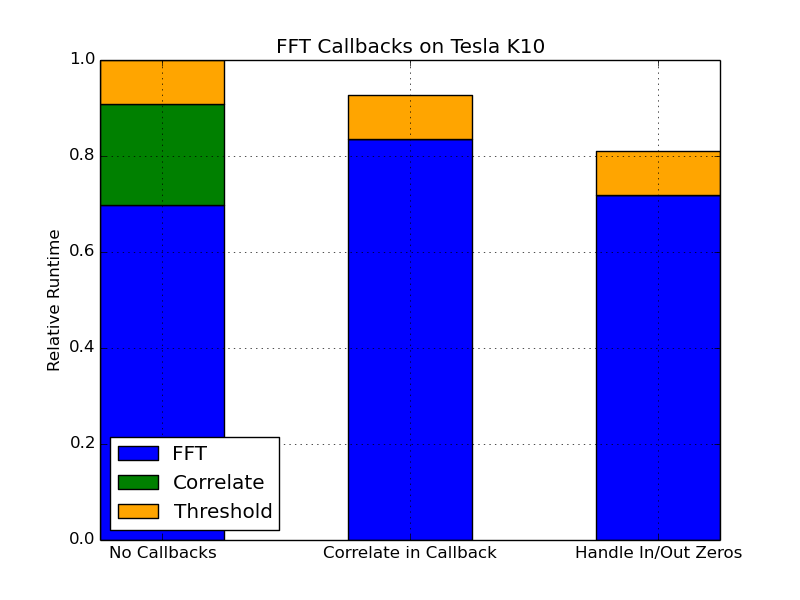
\includegraphics[width=150mm]{plots/callback.png}
\caption{\label{fig:callback} 
The relative performance of the kernels that make up the critical inner loop of the 
matched-filtering code. (Left) The initial GPU kernel implementations without the
use of cuFFT callbacks. (Middle) Naive fusion of the correlate into a load callback.
(Right) Fusion of the correlate kernel into the load callback, where memory reads
are avoided where the input is known to be zeros, and output writes are avoided
where it is known to be corrupted by wrap-around effects.
}
\end{figure}

\subsubsection{Future Safe Optimizations}
% Hopefully move many of these into the implemented ones which we can then compare in this sections.
% Add more about the drawbacks (inflexibility) of some of these choices
\begin{enumerate}
\item Store template as a real vector of phase values.

For certain kinds of commonly used waveform template, in particular the TaylorF2
approximant, the amplitude of the waveform is a simple power series. This allows
it to be precomputed, and instead of including it with the template itself can be
pre-multiplied into the segment of data to analyze. Where this is possible, the
remaining portion of the template can be expressed in the form $e^{i\psi(f)}$. It is
possible to trade floating point operations for a savings in global memory reads
by storing only the fourier phase of the template, $\psi(f)$, and recalculating
the full $e^{i\psi(f)}$ within a load callback.

\item Store output as real values 

Alough a full analysis does require both the full phase and amplitude information 
of our complex SNR timeseries, it is possible to store the immediate output 
of the inverse FFT only as a series of real values. This can be done, as long
as the current time-frequency signal-constistency test remains the preferred 
method. This test's implementation allows efficient recalculation of the SNR,
including the phase information, at points identified above threshold. This 
storage method would allow savings both the in the required memory writes from
the inverse FFT, but also the memory reads required by the thresholding and 
clustering kernel. 

\end{enumerate}

\subsubsection{Future Speculative Optimizations}
% These  we need to carefully test and may need to work with
% NVIDIA on. 
These are currently unimplemented optimizations that may lose precision but
can be tested using the current cuFFT callback API.

\begin{enumerate}
\item Store Input in FP16 format
\item Store Output in FP16 format
\end{enumerate}


\subsubsection{Optimizations Requiring Additional cuFFT Interfaces}
These are potential optimizations that require features beyond the current callback API
system.

\begin{enumerate}
\item Store intermediate FFT sub-kernel storage in FP16 format

So far, the callback APIs support adding load and store functions for only the initial
and final vectors, not for intermediate data products. Performing the FFT operations
in FP32 and storing the intermediate products in FP16 may be possible. We are beginning
a study to determine if this model could meet our accuracy requirements.

\item Merge the threshold clustering algorithm into the final FFT kernel

If the callback API can be extended to allow a vectorized version of the store callback
that operates on contiguious elements, it may be possible to merge a portion of the
peak finding algorithm into the store callback, vastly decreasing the memory writes.

\end{enumerate}

\subsubsection{Kernel Launching and Host interaction}

In the previous sections, we have focused on making optimal use of GPU's resources. As GPU kernels
launches are aynchronous compared to host execution, it is possible to hide trivial serial operations
that occur within the host-code. The exception is where triggers are offloaded from the GPU onto the CPU.
Host execution does not proceed as the GPU queue is drained. When the data is synchronized there
is a noticeable delay before new GPU kernels are executing. This can be minimized by executing
multiple host processes that submit work to the same GPU, and by batching additional work together
to amortize the device offload latency.


\subsection{Implementation on Intel MICs}
I do not know if we have investigated this much at all---how much work to add a
``mic'' processing scheme to pycbc, and start investigating its performance? It
is possible that we can simply carry over the strategies from the CPU section,
just ensuring we benchmark on a MIC as well.  FFTW does not support MIC, so we
will only be testing MKL there, presumably.


\section{Sub-component Benchmarks}
\label{sec:benchmark}

Our plan here is to benchmark on several specific pieces of hardware.  For most
of these, we will probably try to benchmark both specific kernels in isolation,
to verify that their performance matches the theoretical prediction from
section~\ref{sec:search_methods}, as well as the full matched filter itself, on
different representative data methods. 

\subsection{Various GPUs}

Specific GPUs on which to benchmark:

\begin{enumerate}
\item K10 (at CIT)
\item GTX 980 (at Syracuse)
\item GTX 750 (at Atlas)
\end{enumerate}

\subsection{Various CPUs/MIC}

Specific CPUs to benchmark:

\begin{enumerate}
\item Intel E5-2670v2 (CIT Sandy Bridge)
\item Intel E5-2699v3 (CIT pcdev11); or do we want to acquire another Haswell
  but with a 20 MB cache?
\item Intel E3-1231v3 (``newer'' Atlas Haswells; 8 MB cache)
\item Intel E3-1220v3 (``older'' Atlas Haswells; also 8 MB cache).
\end{enumerate}

\section{In-situ benchmarks}

\section{Conclusions}
\label{sec:conclusions}

\section{Acknowledgments}
\label{sec:acknowledgments}

% References
\bibliographystyle{unsrt}
\bibliography{../../../bibtex/cbc-group}{}

\end{document}
